\section{编程范式}
\label{sec:paragigms}

\begin{frame}
  \begin{center}
    \Huge{\textcolor{red}{编程范式}}
  \end{center}
\end{frame}

\subsection{编程范式}

\begin{frame}{主流编程范式}
    \begin{enumerate}
    \item \alert{指令式}: Imperative Programming
    \item \alert{函数式}: Functional Programming
    \item \alert{逻辑式}: Logic Programming
    \item \alert{面向对象}: Object Oriented Programming
    \end{enumerate}
\end{frame}

\subsection{OO与FP}

\begin{frame}{大师互殴}
  \begin{figure}
    \centering
    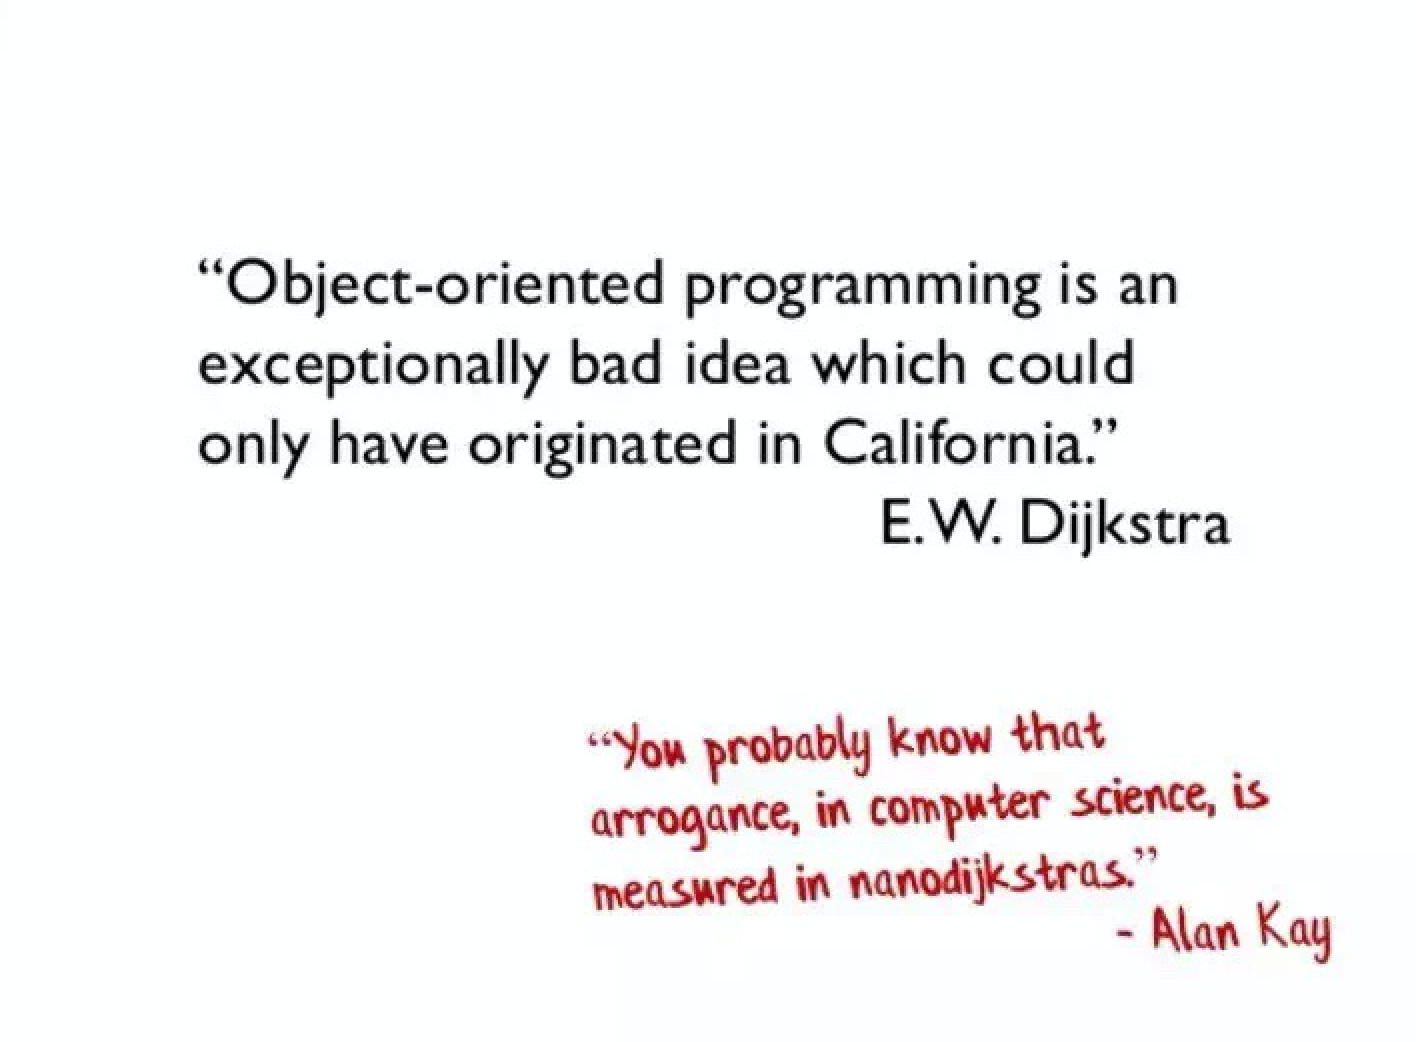
\includegraphics[width=0.7\textwidth]{oovsfp.png}
  \end{figure}
\end{frame}

\begin{frame}{不公开的较量}
  \begin{figure}
    \centering
    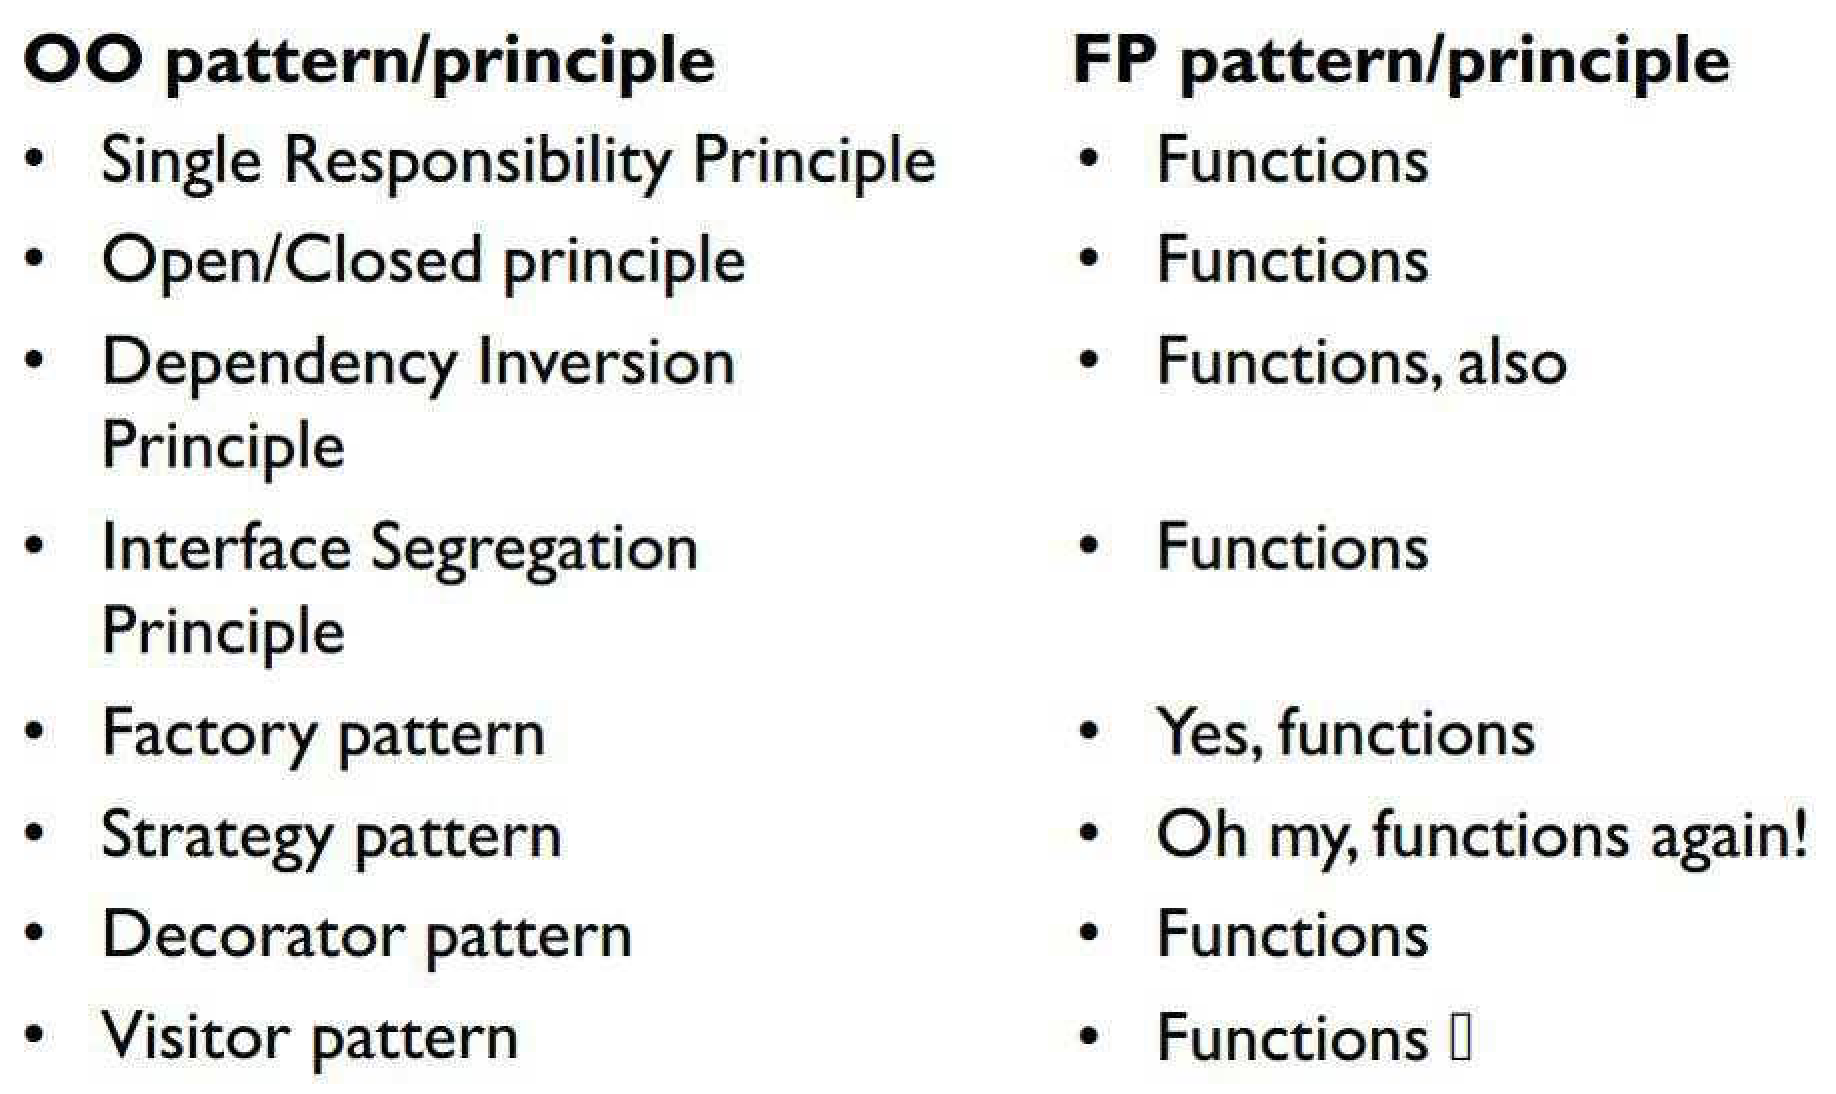
\includegraphics[width=0.7\textwidth]{fpvsoo.png}
  \end{figure}
\end{frame}

\subsection{Scala}

\begin{frame}{Scala = OO + FP}
    \begin{itemize}
    \item \alert{自由的}
    \item \alert{开放的}
    \item \alert{简洁的}    
    \item \alert{高阶的}
    \end{itemize}
\end{frame}
